\chapter{Umsetzung}
\label{chap:data_collection}
Für die Umsetzung wurde auf Bild \ref{fig:inhalt_semesterarbeit} Inhalt der Semeseterarbeit dargestellt folgende Schritte durchgeführt:

\begin{itemize}
  \item erstellen docker-compose Datei
  \item Anpassung der detect-hate.com App
  \item Pipelines in Streamsets erstellen
\end{itemize}

Das Vorgehen für die Umsetzung ist iterativ, da Datenbanken, Indexes, und das Dashboard einen Einfluss auf die einzelnen Schritte in der Pipeline hatte:


 es wurde mit einfachen Pipelines begonnen um einen ersten Durchstich zumachen und anschliessend wurden Verbesserungen an den Pipelines und Software Konfigurationen vorgenommen.

da es immer wieder Anpassungen an den Pipelines, Elasticsearch Indexs und den Dashboard gab, wie zum Beispiel: 

Anpassung der Pipeline "detect tweets": 
\begin{itemize}
  \item Einfügen eines weiteren Schrittes um Atttribute aus dem json zu entfernen, weil der Elasticserach Index zu gross wurde 
  \item 
\end{itemize}

\section{Docker-compose file }
\label{sec:docker_compose}

\textbf{Aufbau}
todo: Beschreiben

\textbf{Volumes}

F{\"u}r die Datenhalten gibt es in Docker unterschiedliche Varianten: Es besteht die M{\"o}glichkeit die Daten im Docker container selber oder ausserhalb din einem sogenannten persistenten Speichervolumen abzulegen. F{\"u}r diese Semesterarbeit wir auf solche Speichervolumen zur{\"u}ckgegriffen. 

Warum persistente Speichervolumes verwenden?

Container sind verg{\"a}nglich und haben ein eigenes Dateisystem.  Wenn Container sterben, sind auch die lokal in ihrem Dateisystem gespeicherten Daten verschwunden. Dies bedeutet f{\"u}r zustandsabh{\"a}nngige Anwendungen wie MySQL oder MongoDB oder PostgreSQL, dass die gespeicherten Daten verlohren sind, sobald ein Container abst{\"u}rzt, stirbt oder gel{\"o}scht wird. Die Daten sind in den oben genannten Anwendungen zentral und d{\"u}rfen nicht verloren gehen, unabh{\"a}nngig vom Zustand den Containers.

Was ist ein persistentes Speichervolumen?

Eine Speichervorrichtung oder ein Datentr{\"a}nger, der einen Containerabsturz oder seinen Lebenszyklus {\"u}berstehen kann, wird als Persistent Storage Volume bezeichnet. Persistente Speichervolumen k{\"o}nnen auf
\begin{itemize}
  \item einer Festplatte erstellt werden, die direkt auf der Host-Maschine installiert ist 
  \item einem NAS-Speichervorrichtung im lokalen LAN-Netzwerk erstellt werden
  \item einer Cloud-Speichervorrichtung erstellt werden
\end{itemize}
unter der Voraussetzung das sie auf der Host-Machine verf{\"u}gbar sind.

Es gibt zwei verschiedene Methoden, um ein persistentes Speichervolumen in einen Docker Container einzubinden.

Variante 1:

Erstellen eines neuen persistenten Speichervolumens auf der Host-Maschine und dieses in einem Ordner innerhalb eines Docker-Containers mounten. Der Docker Container erh{\"a}nlt exklusiven Zugriff auf das Speichervolumen. Die im Volume gespeicherten Daten k{\"o}nnen nicht einfach von der Host-Maschine aus gelesen, manipuliert oder besch{\"a}ndigt werden.
  
Variante 2:

In den Docker Container einen lokalen Ordner des Hostcomputers einbinden, so dass Daten zwischen dem Hostcomputer und dem Docker Container ausgetauscht werden k{\"o}nnen. Diese Methode ist sehr n{\"u}tzlich, wenn der Host-Computer auf die Daten oder die Datenbank zugreifen oder regelm{\"a}nßig sichern m{\"o}chte, die vom DB-Server, der im Docker-Container l{\"a}nuft, in den Ordner geschrieben wurden.

In dieser Semesterarbeit wurde Variante 1 gew{\"a}n{\"a}nhlt, da erstens ein Zugriff vom Host nicht n{\"o}tig ist und zum Zweiten der Container ohne gr{\"o}ssere Anpassungen auf einem anderen Host laufen soll. Bei Variante 2 m{\"u}sse das docker-compose.yaml angepasst werden.

Volumes werden wie folgt erstellt:

\begin{lstlisting}[float=h,frame=tb,caption={Befehl zum Volume erstellen},label=lst:erstelle_volume]
		{docker volume create --name=mongodb}
\end{lstlisting}  

Ben{\"o}tigte Tools in file Eintragen (hier in der Dokumentation exemplarisch f{\"u}r MongoDB, docker-compose.yaml imd Anhang zu finden)

\begin{lstlisting}[float=h,frame=tb,caption={Auszug docker-compose.yaml MongoDB},label=lst:mongo_docker]
		{## MongoDB
			mongodb:
   				image: mongo:4
   				container_name: mongodb
    				ports:
      				- 27017:27017
    				environment:
      				- MONGO_INITDB_DATABASE=database
      				- MONGO_INITDB_USERNAME=user
      				- MONGO_INITDB_PASSWORD=password
   			 	volumes:
      				- mongodb:/data/db
    				restart: always}
\end{lstlisting}  

Verwendete Volumes im file angeben:
\begin{lstlisting}[float=h,frame=tb,caption={Auszug docker-compose.yaml zum Volume erxtern},label=lst:extern_volume]
		{volumes:
  			mongodb:
    				external: true}
\end{lstlisting}  

Nach dem Erstellen der docker-compose.yml Datei kann mit einem Befehl gepr{\"u}fen werden ob die Datei korrekt ist \ref{lst:check_yml}:
\begin{lstlisting}[float=h,frame=tb,caption={Befehl um .yml auf Korrektheit zu pr{\"u}fen},label=lst:check_yml]
		$docker-compose -f filename config
\end{lstlisting}

Problem mit local host testen: Aus dem Docker raus geht das nicht so einfach

\section{Software konfigurieren}
\label{sec:tool_konfigurieren}

\subsection{Docker Container starten}
Einrichten der Variablen.
\begin{lstlisting}[float=h,frame=tb,caption={Befehl um Docker Container zu starten},label=lst:docker_up]
		$export DOCKER_HOST_IP=xxx.xxx.xxx.xxx
		$export PUBLIC_IP=xxx.xxx.xxx.xxx		
		\end{lstlisting}

Docker Container mit dem Befehl von \ref{lst:docker_up} starten.
\begin{lstlisting}[float=h,frame=tb,caption={Befehl um Docker Container zu starten},label=lst:docker_up]
		$docker-compose up
\end{lstlisting}

\subsection{Kafka}


\subsection{MongoDB}


\begin{lstlisting}[float=h,frame=tb,caption={Befehl um Docker Container aufzurufen und MongoDB shell au starten},label=lst:docker_call_mongo]
		$docker exec -ti mongodb mongo
\end{lstlisting}

\begin{lstlisting}[float=h,frame=tb,caption={Befehl um zur tweets Datenbank zu wecheln},label=lst:chnage_db]
		>use tweets
\end{lstlisting}

\begin{lstlisting}[float=h,frame=tb,caption={Befehl um Tweet Dokumente in  Tweets Collection zu schreiben},label=lst:insert_collection]
db.tweets.insert({
  "created_at":"Tue Aug 06 19:08:09 +0000 2019",
  "id":1158817051458298224,
  "id_str":"1158817051458228224",
  "text":"@dinodlz @KLGLASS2 He isn’t welcome. But when has that ever stopped trump from doing what he  	wants? Knowing he is i… ,
  ......
  "lang":"en","timestamp_ms":"1565118489504"
})
\end{lstlisting}


\subsection{Elasticsearch}
Verwendung der REST-API
Sobald eine ElasticSearch Instanz in Betrieb ist, kann diese über eine JSON-basierte REST-API angesprochen werden. Die Kommunikation kann mit jedem beliebigen HTTP-Client erfolgen. In der Dokumentation von ElasticSearch wird in allen Beispielen Curl verwendet, aber es ist auch möglich einen grafischen Client wie den RESTClient zu verwenden. 

Prüfen ob der Service verfügbar ist mit: http://lokalhost:port/

\begin{lstlisting}[float=h,frame=tb,caption={Befehl ein Dokument in Elasticsearch einzufügen},label=lst:elastic_creat_doc]
curl -H "Content-Type: application/x-www-form-urlencoded" curl 
-XPUT 'http://192.168.178.127:9200/predictedtweets' -d "{
   "mappings": {
     "_id": ObjectID("5d5ae74d9494be000153670e"),
     "created_at": "Mon Aug 19 17:55:14 +0000 2019",
     "id": "1163504741898874882",
     "text": "RT @realDerekUtley: Retweet if you think @SenatorSandoval should resign
      for staging an assassination of @realDonaldTrump,
     .......
     },
   	.......
     "prediction": {
         "predictions": {
             "Linear_SVC": "abusive",
             "Logistic_Regression": "not abusive",
             "Multinomial_NB": "abusive",
             "lstm": "not abusive"
         },
         "probabilities": {
             "Linear_SVC": "69.38%",
             "Logistic_Regression": "62.83%",
             "Multinomial_NB": "72.70%",
             "lstm": "100.00%"
         },
         "probabilities_racist": {
             "Logistic_Regression": "-",
             "down_Linear_SVC": "8.19%",
             "down_Multinomial_NB": "2.50%",
             "lstm": "-",
             "up_Linear_SVC": "0.05%",
             "up_Multinomial_NB": "0.11%"
         },
         "probabilities_sexist": {
             "Logistic_Regression": "-",
             "down_Linear_SVC": "8.88%",
             "down_Multinomial_NB": "2.80%",
             "lstm": "-",
             "up_Linear_SVC": "0.07%",
             "up_Multinomial_NB": "0.04%"
         }
     }
   }
 }"
\end{lstlisting}


\section{Pipeline Architektur}
\label{sec:pipeline_architecture}
In dieser Semesterarbeit setzt sich die Pipeline aus den in Kapitel \ref{sec:streaming} beschriebenen zusammen: 

Streamsets: Bau der Pipelines

Kafka: Verteilen der Tweets

MongoDB: Rohdaten von Twitter für die Masterarbei speichern

Elasticsearch: Bearbeitete Daten von Twitter und Klassifikation speichern

Kibana: Dashboard visualiseren.

\begin{figure}[H]
	\centering
		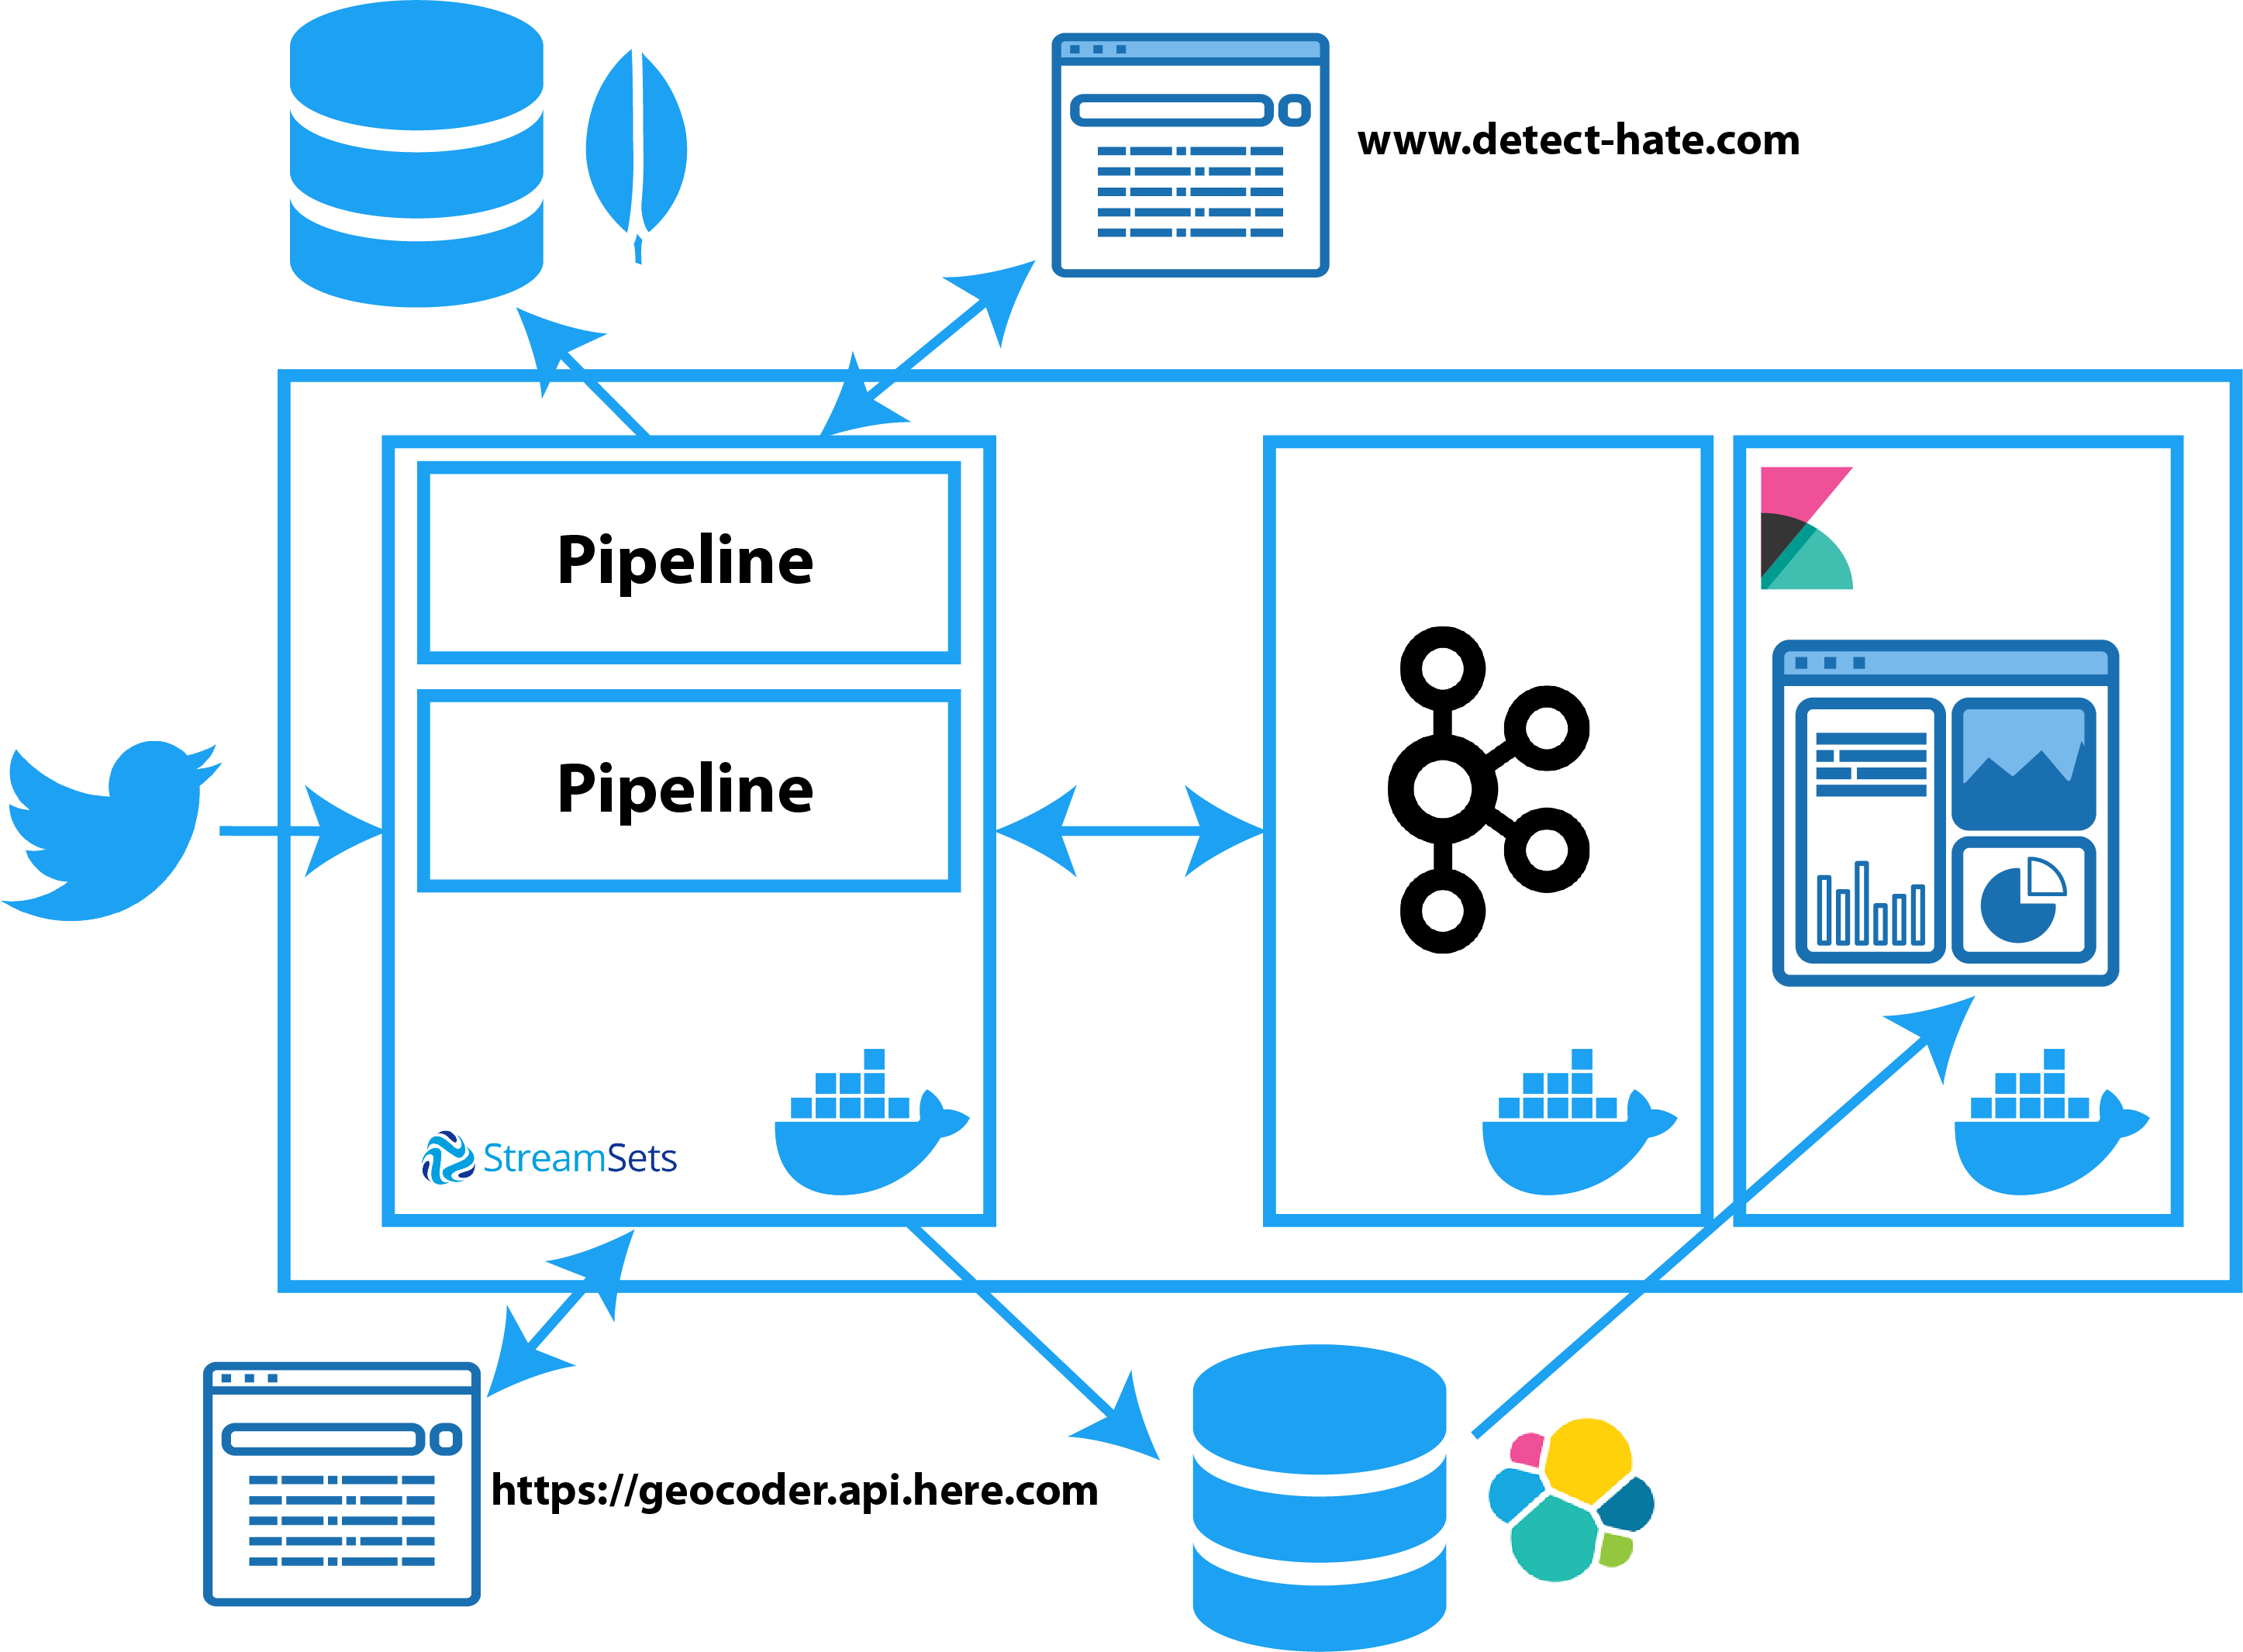
\includegraphics[scale=0.4 ]{images/architecktur_high_level.png}
	\caption{High Level Pipeline Architekttur}
	\label{fig:high_level_architecure}
\end{figure}


todo: Beschrieben warum Mongo Pipeline seperat und nicht mit predict in einem. Ist weil datensammlung für Masterarbeit unabhängig laufen soll. Änerungen an Pipline sind nur möglich wenn die pip  gestoppt  wird. Da des öfteren Anpassungen an der preditct pip gemacht werden müssen, würde so jedesmal die mongo pip gestppt.

Für die Umsetzung, siehe \ref{fig:high_level_architecure} wurden pro abzuarbeitender Einheit eine eigene Pipeline erstellt. Die Kommunikation zwischen den Pipelines erfolgt mittels Kafka mit je separaten Topics. 

Dies wurde so gemacht, dass die Schritte gekapselt sind und Änderungen an den einzelnen Pipelines gemacht werden können ohn e 


\begin{figure}[H]
	\centering
		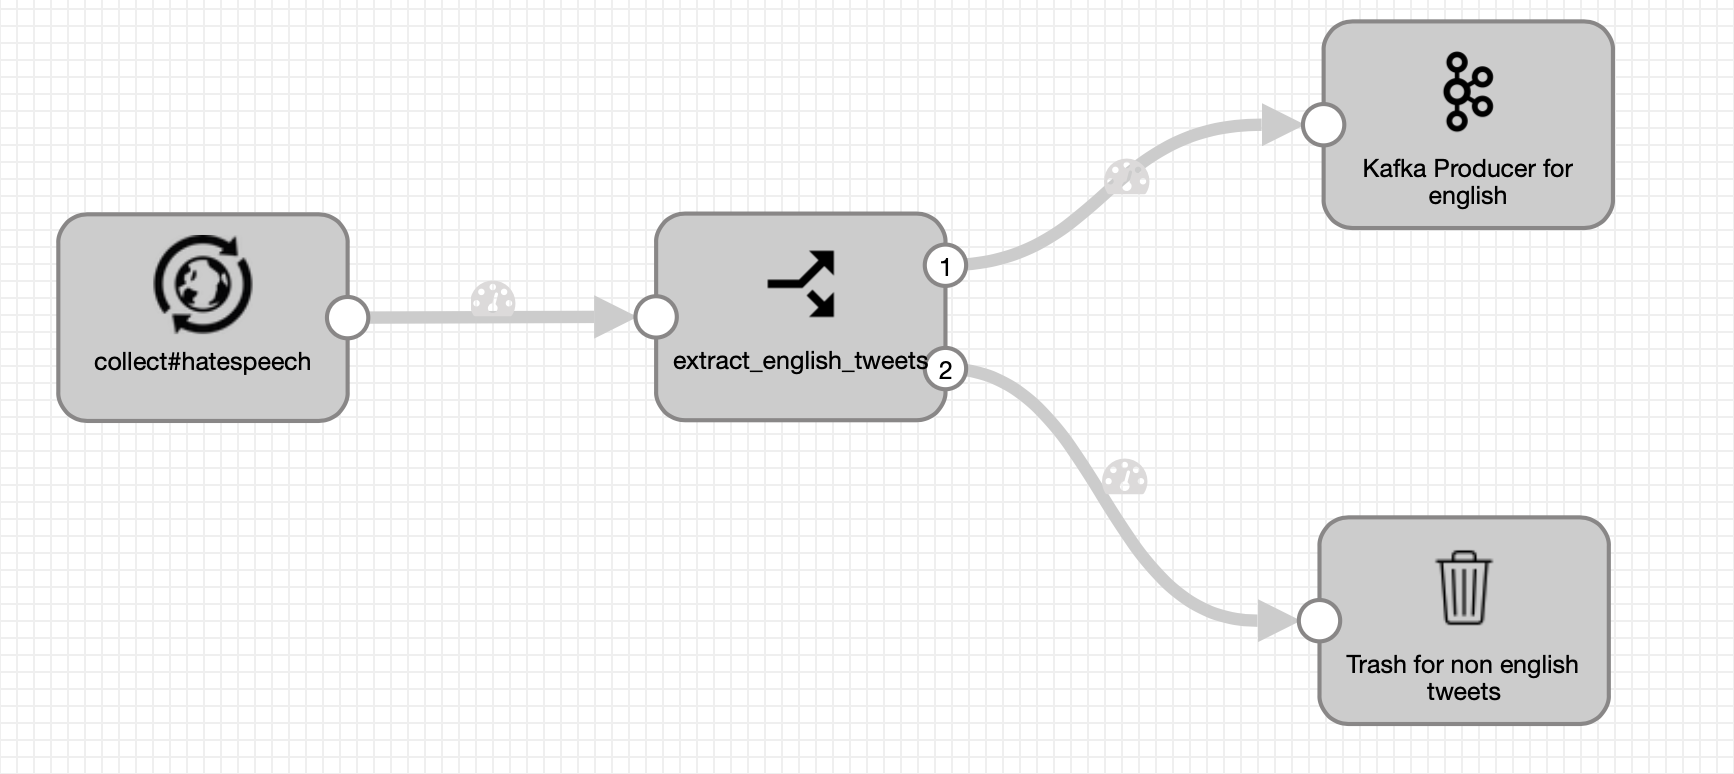
\includegraphics[scale=0.4 ]{images/collect_tweets.png}
	\caption{Pipeline um Daten von Twitter zu bekommen}
	\label{fig:high_level_architecure}
\end{figure}

\begin{figure}[H]
	\centering
		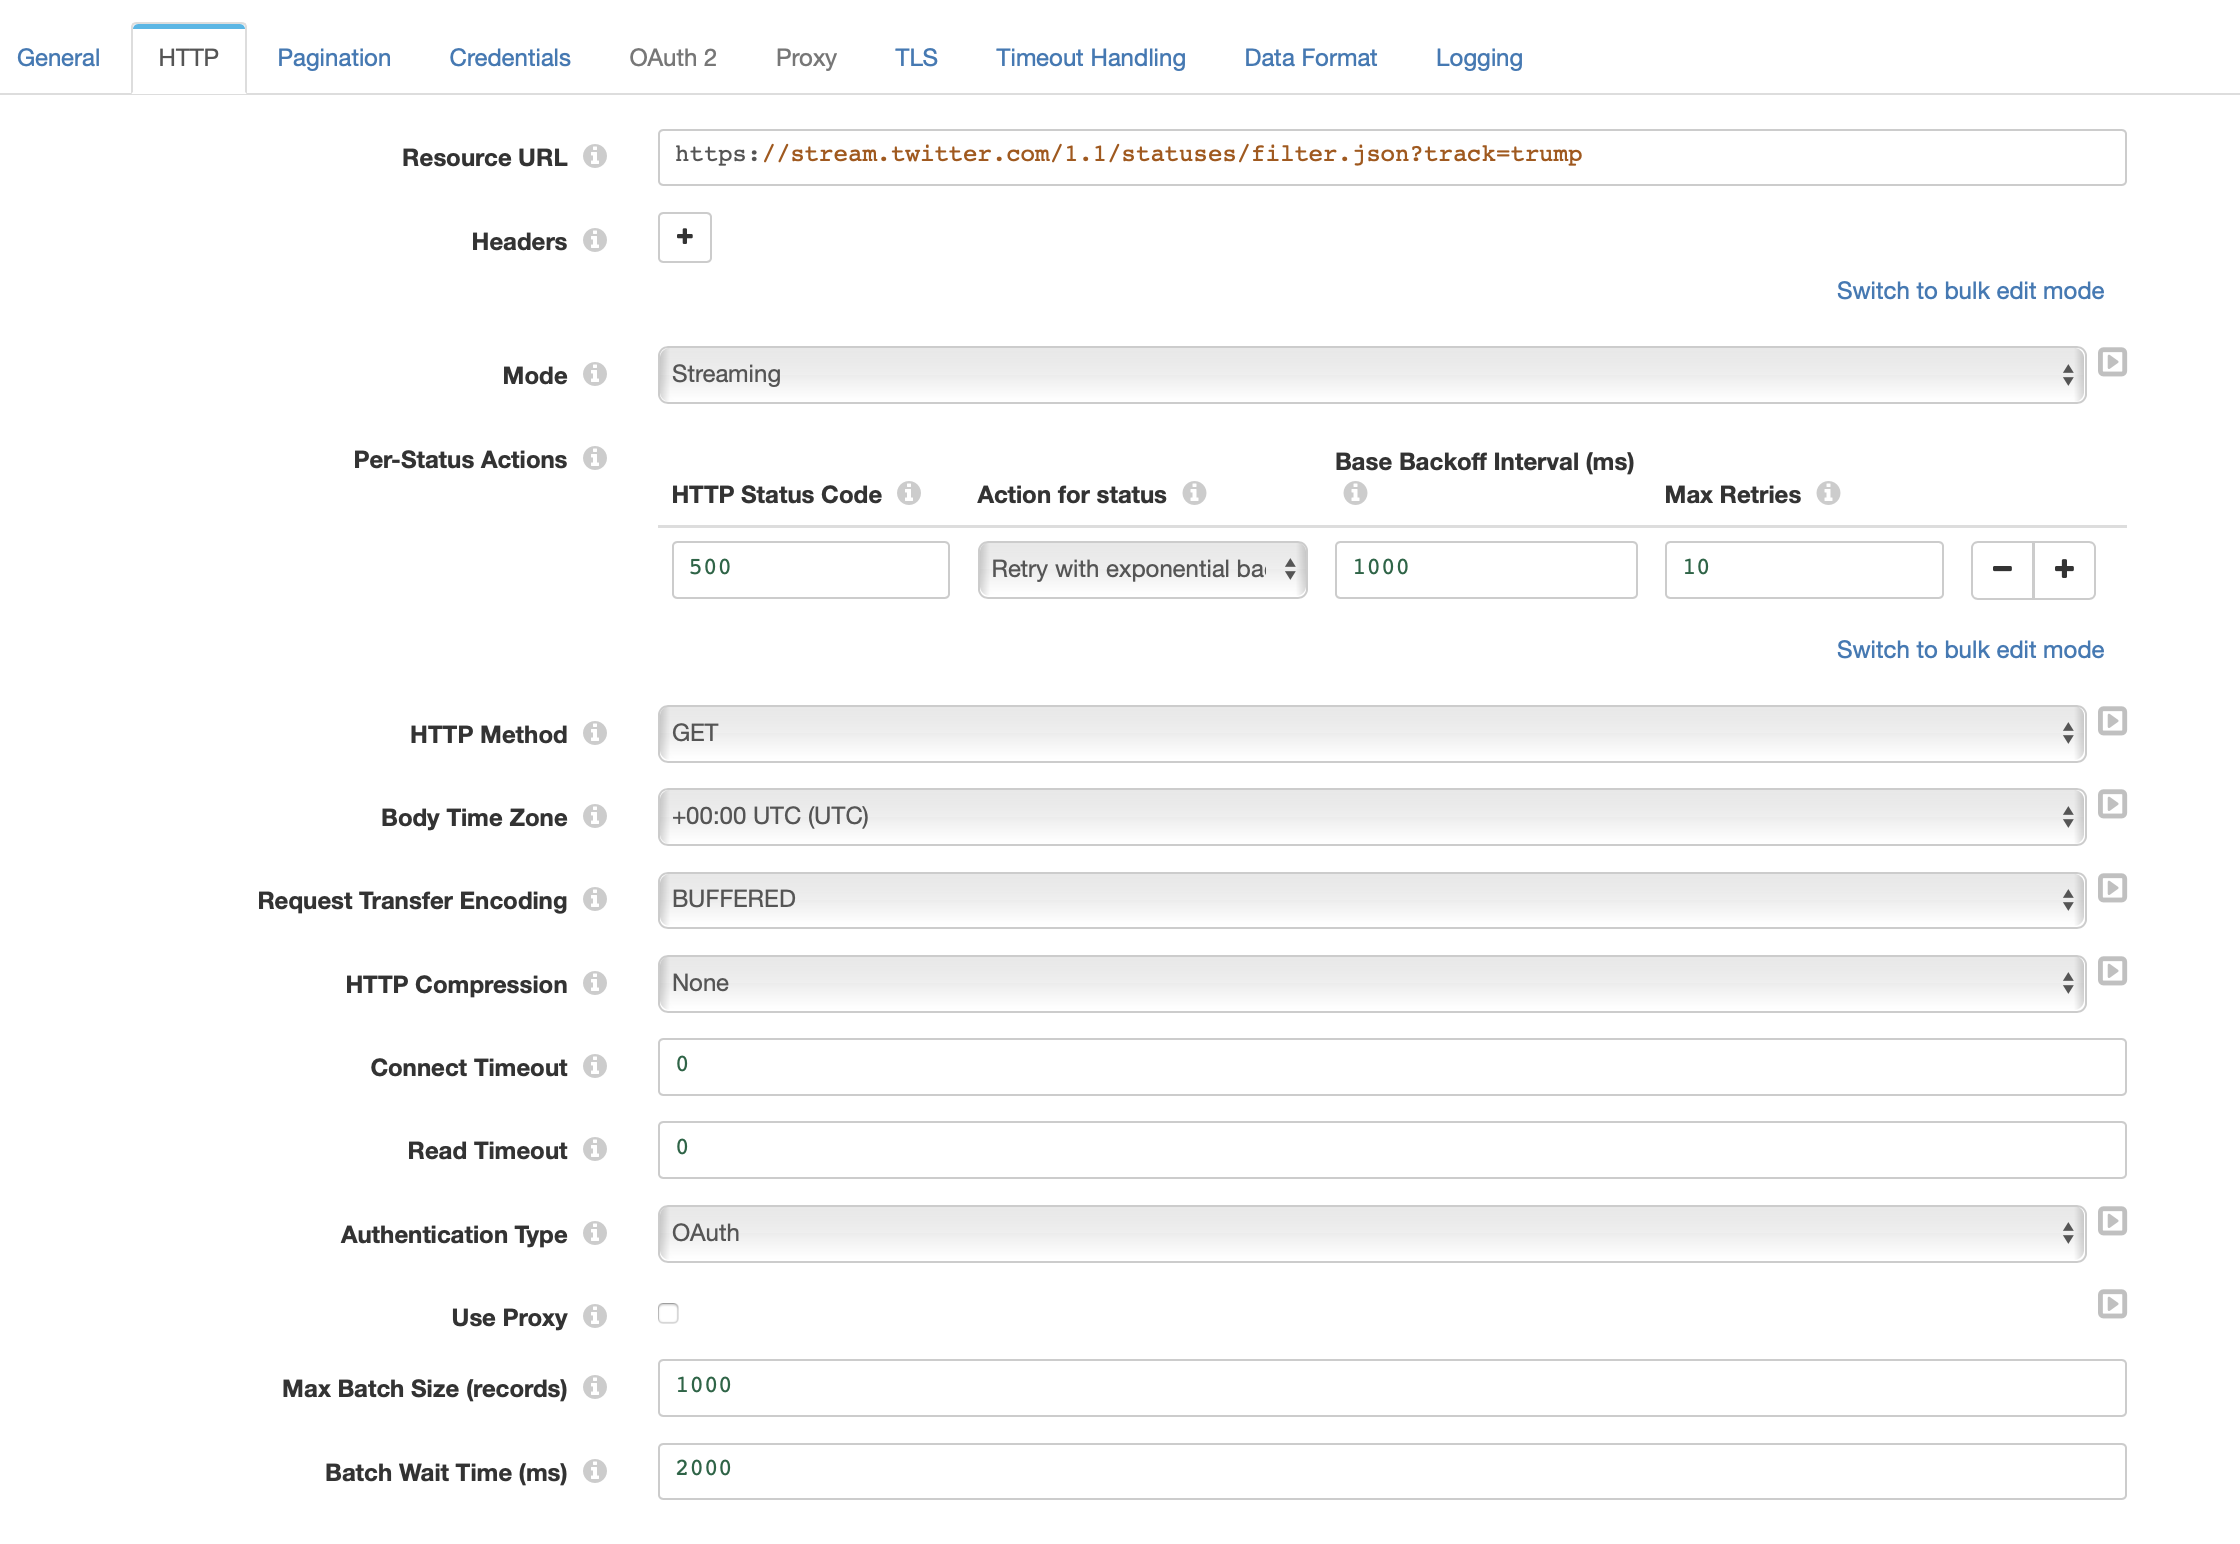
\includegraphics[scale=0.4 ]{images/settings_twitter.png}
	\caption{HTTP Client Settings }
	\label{fig:high_level_architecure}
\end{figure}

\begin{figure}[H]
	\centering
		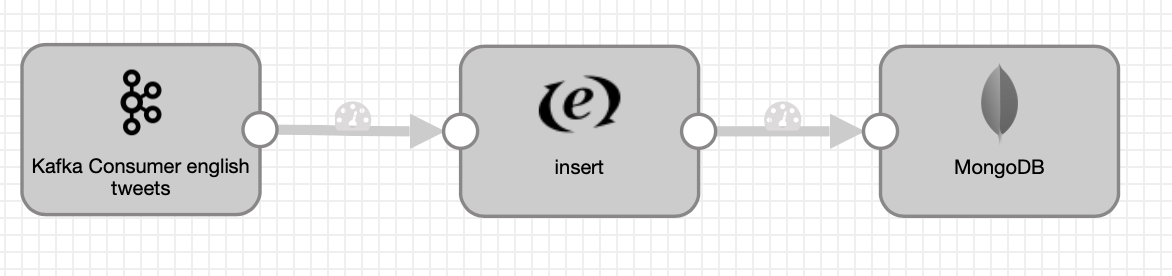
\includegraphics[scale=0.4 ]{images/tweets_to_mongo.png}
	\caption{Pipeline um Daten in MongoDB zu schreiben}
	\label{fig:high_level_architecure}
\end{figure}

\begin{figure}[H]
	\centering
		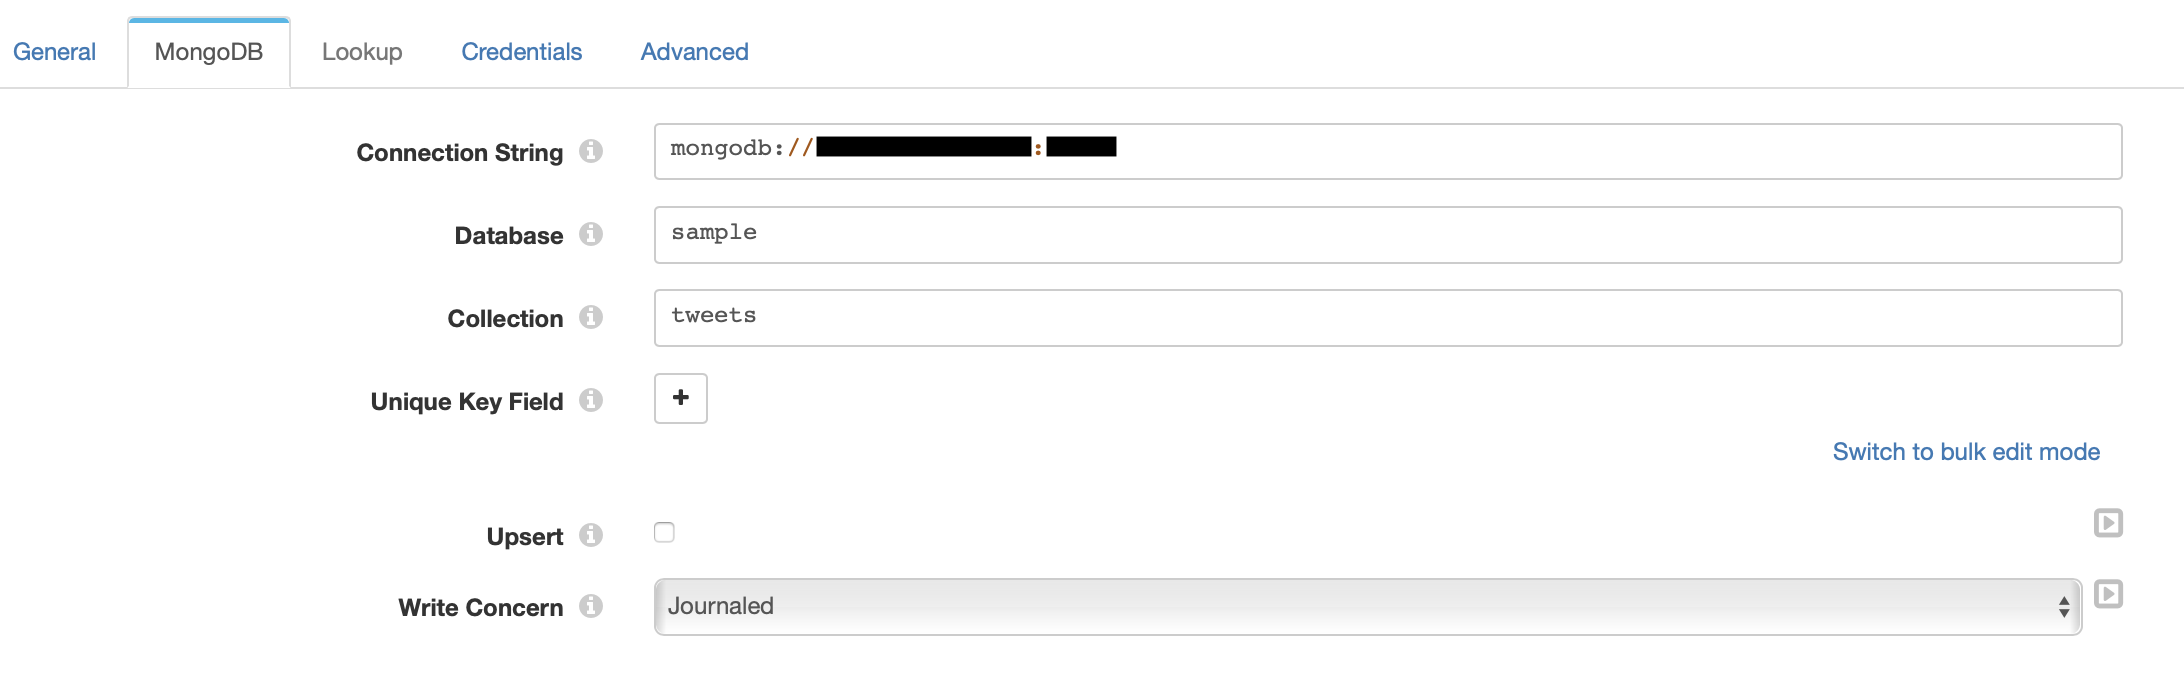
\includegraphics[scale=0.4 ]{images/settings_to_mongo_mongo.png}
	\caption{Settings MongoDB}
	\label{fig:high_level_architecure}
\end{figure}

\begin{figure}[H]
	\centering
		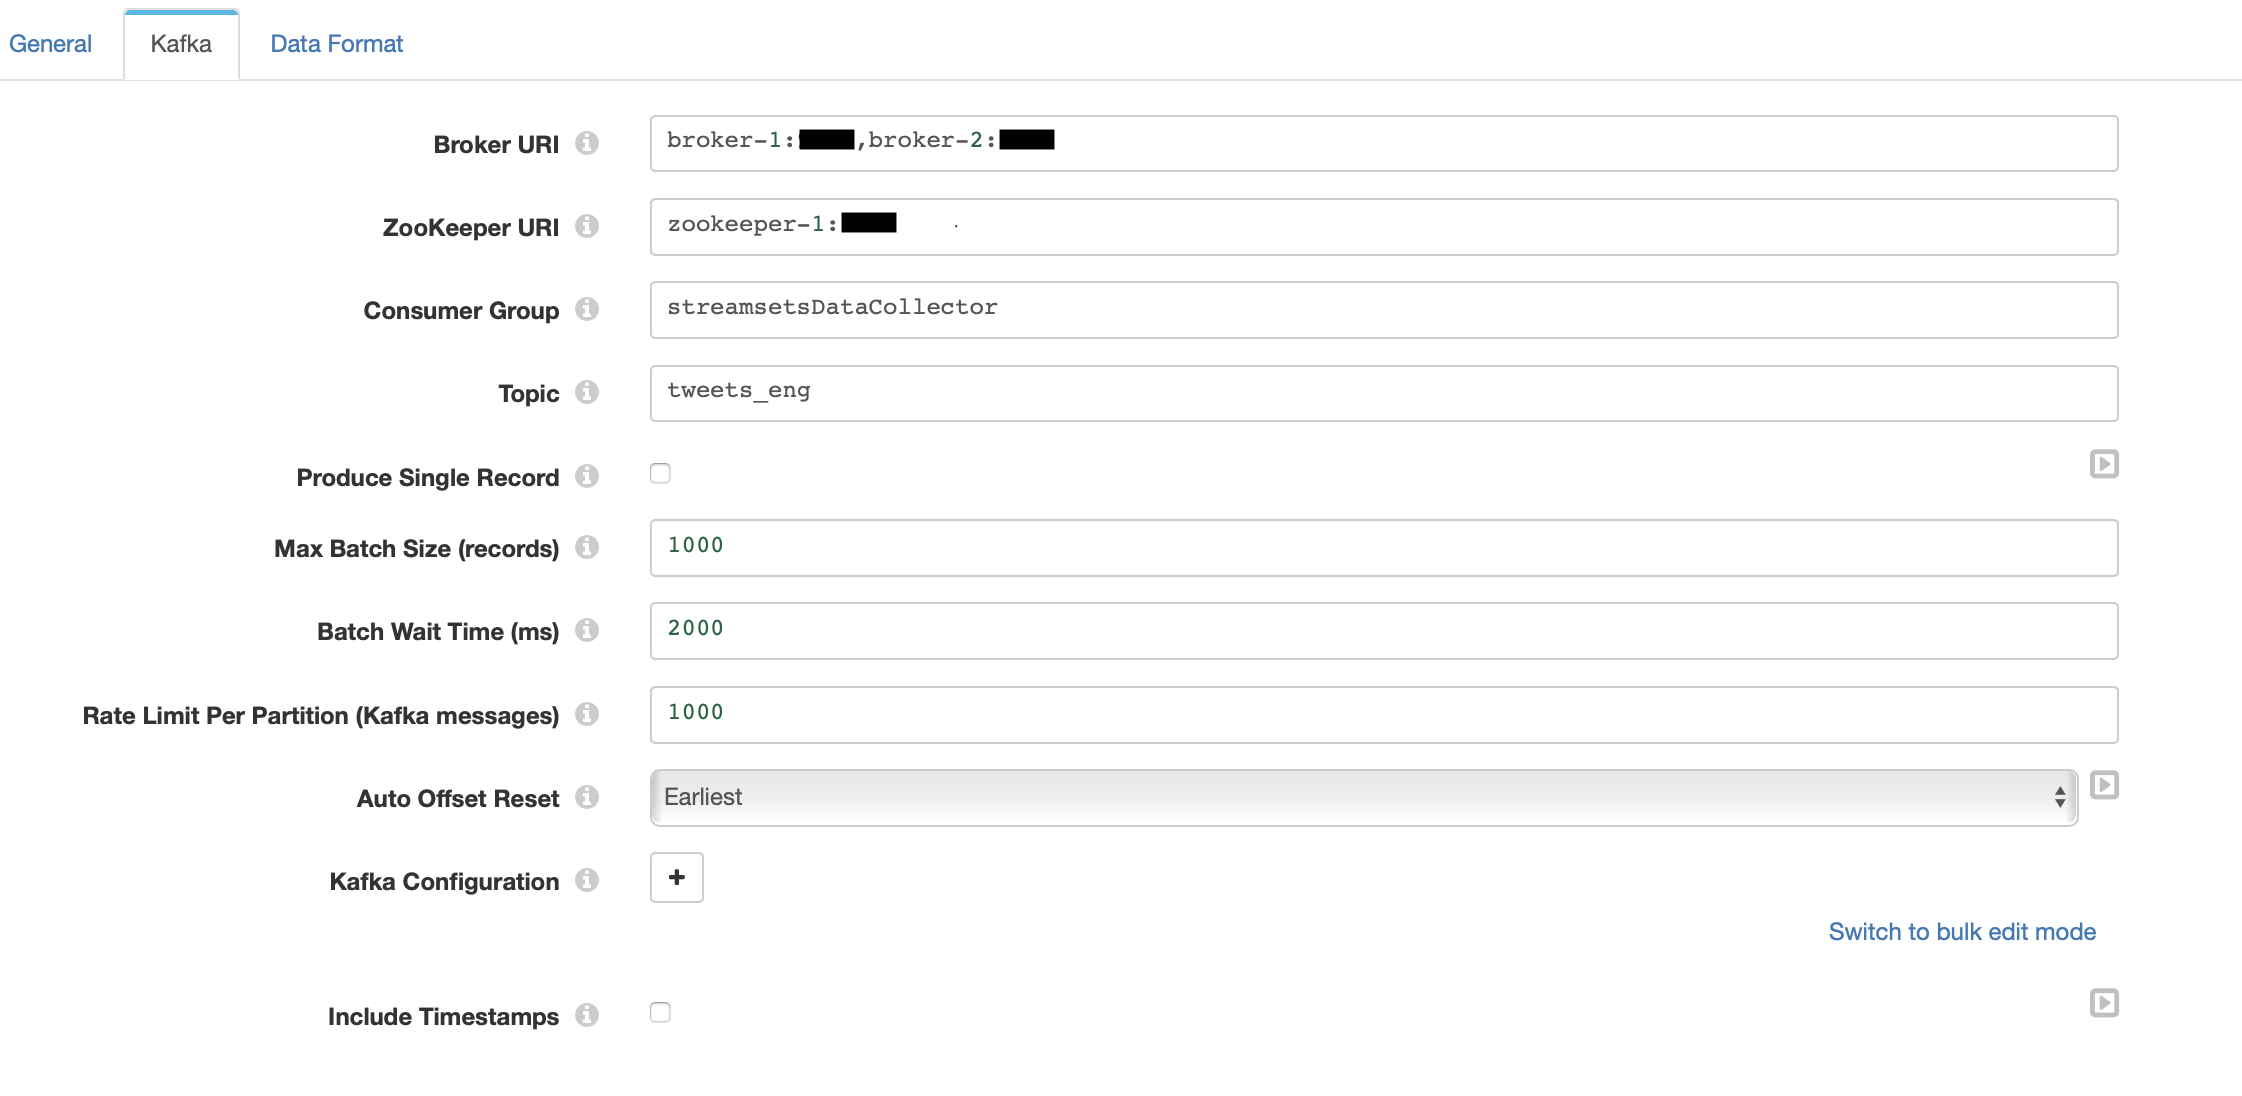
\includegraphics[scale=0.4 ]{images/setting_to_mongo_kafka.png}
	\caption{Settings Kafka Consumer}
	\label{fig:high_level_architecure}
\end{figure}

\begin{figure}[H]
	\centering
		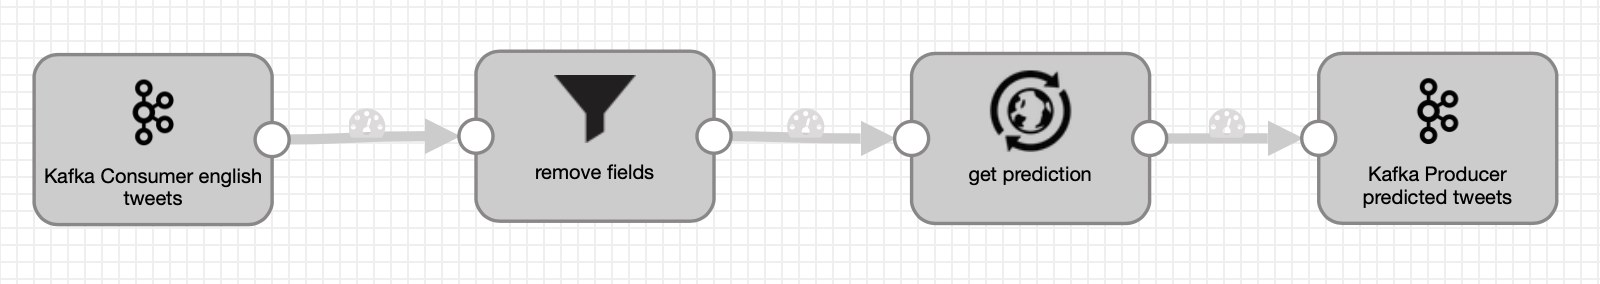
\includegraphics[scale=0.4 ]{images/predict_tweets.png}
	\caption{Pipeline um die Tweets zu klassifizieren}
	\label{fig:high_level_architecure}
\end{figure}

Nach dem die Pipeline zum Klassifizieren erstellt war und die Resultate 

\begin{figure}[H]
	\centering
		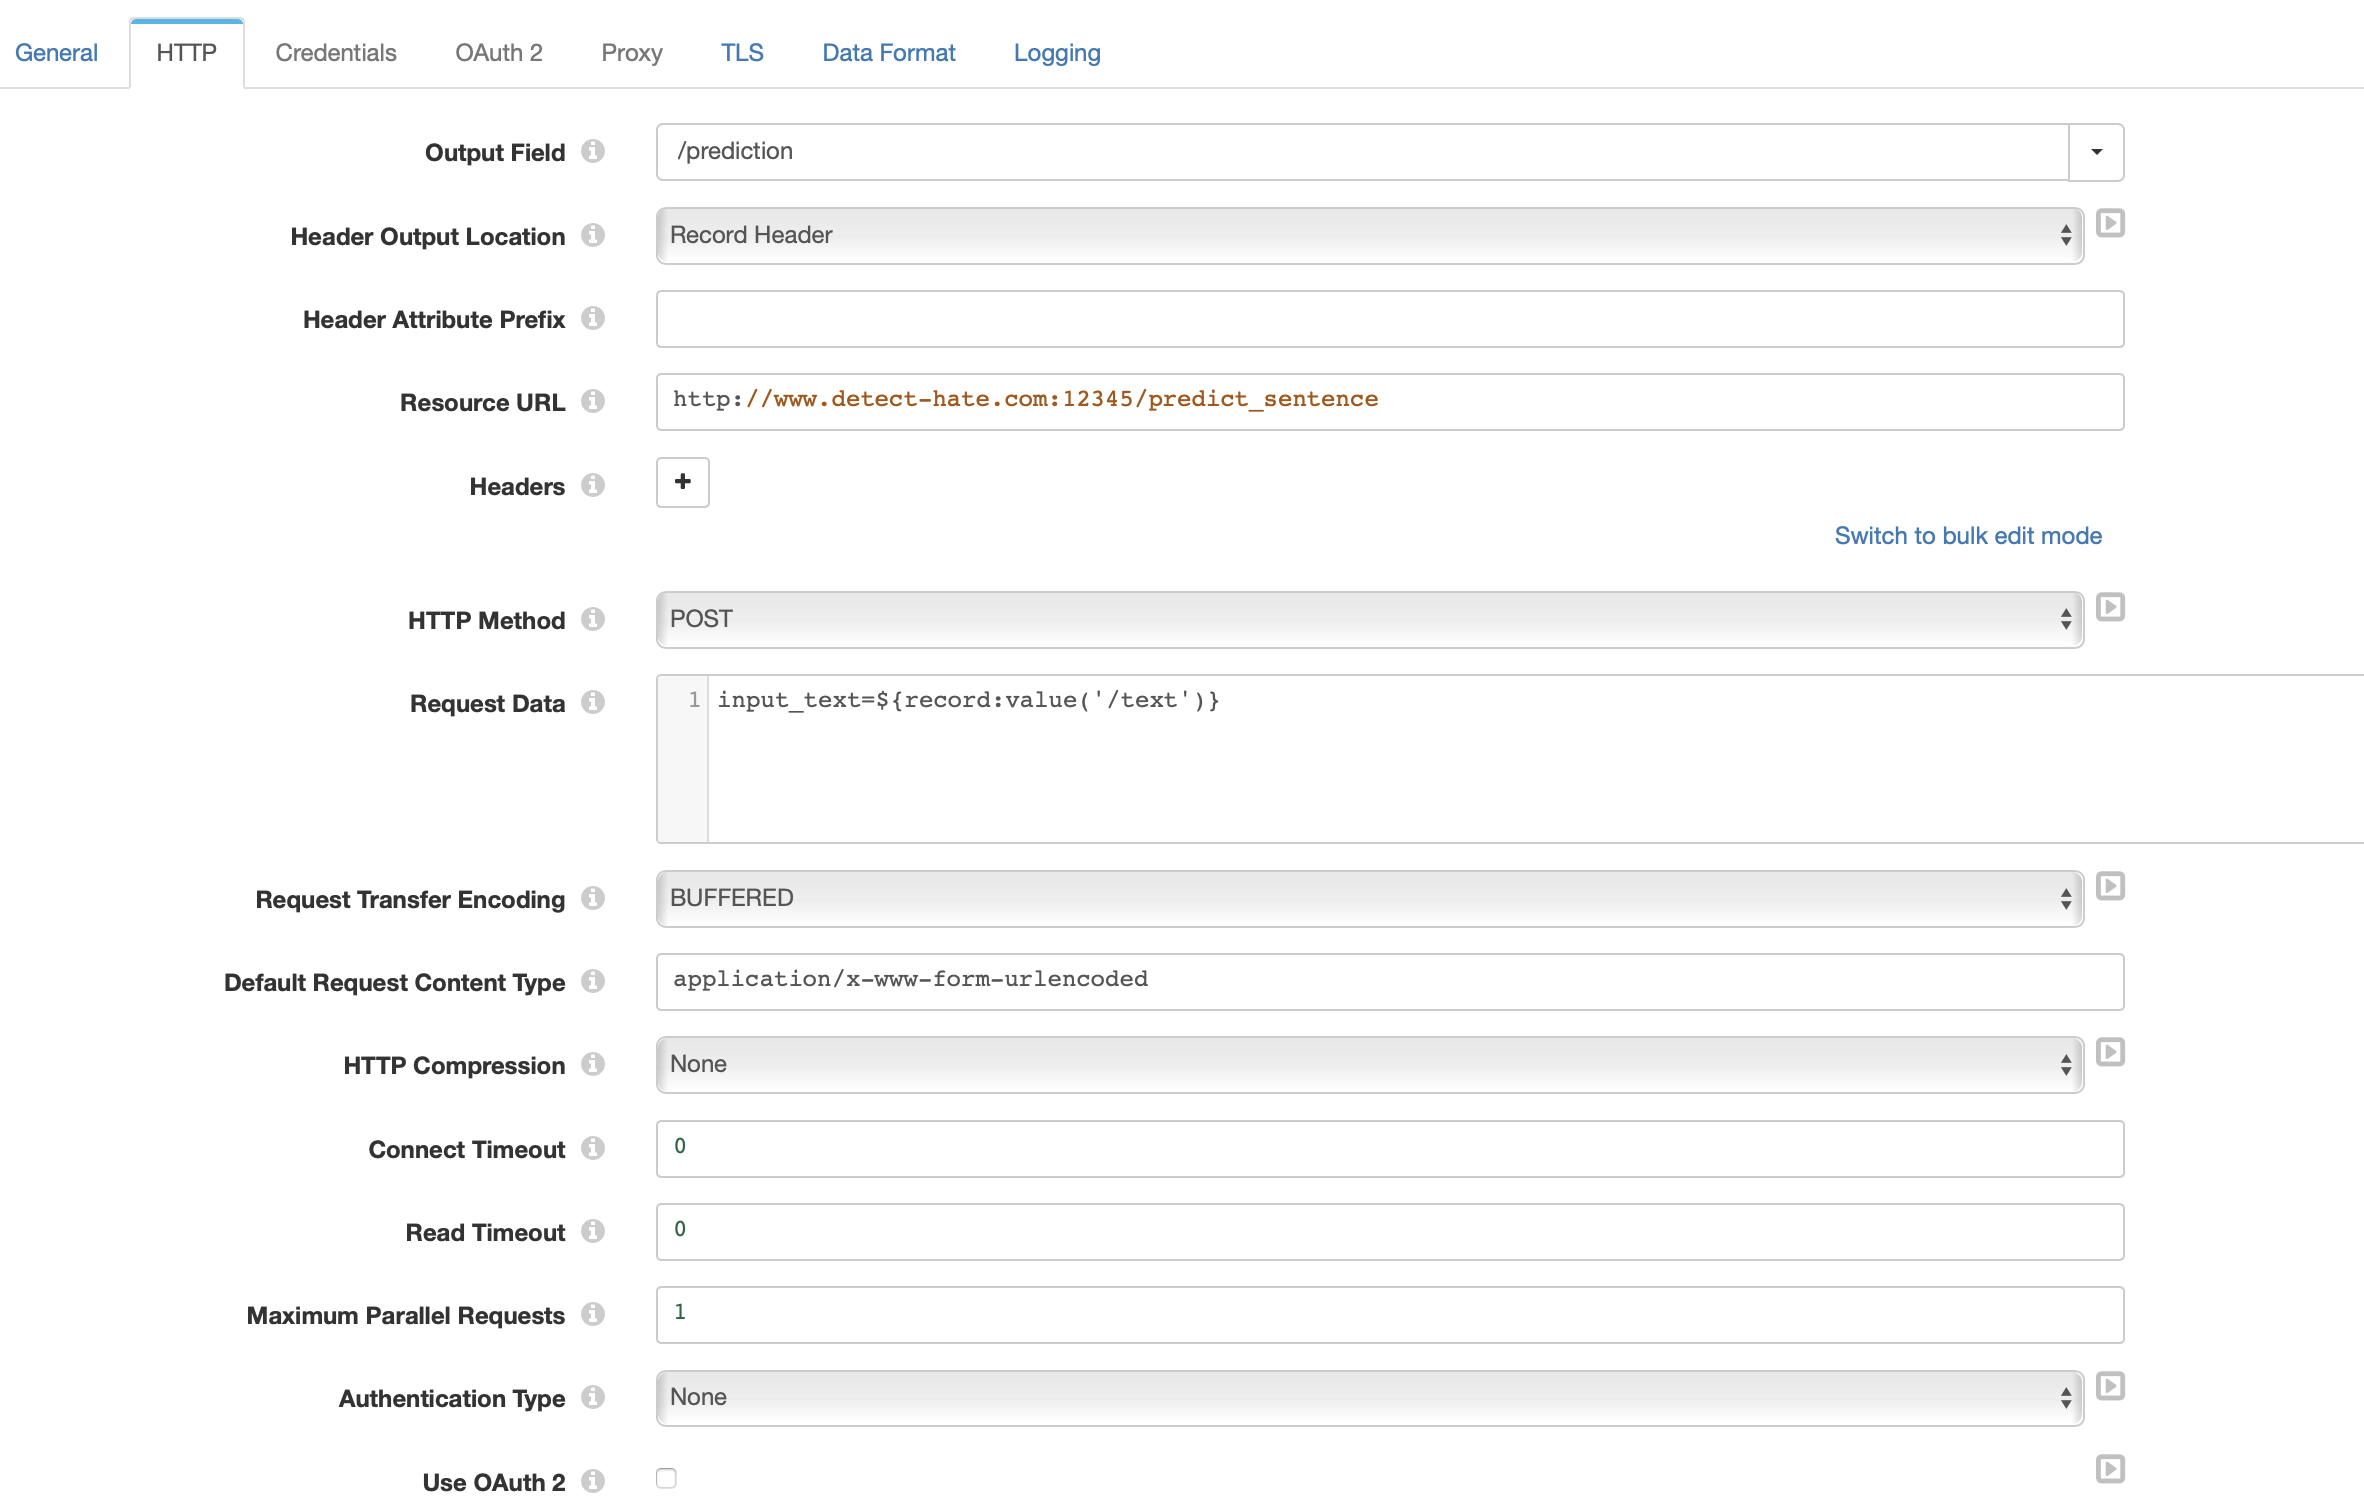
\includegraphics[scale=0.4 ]{images/settings_http.png}
	\caption{Settings HTTP request}
	\label{fig:high_level_architecure}
\end{figure}


\section{Anpassungen an der API}
\label{sec:anpassung_api}

\section{Installation auf dem nHex}
\label{sec:nHex}

Die Spezifikation des BigBoards Cluster "nHex i3" ist in Tabelle \ref{tab:pez_hnex} beschrieben.

\begin{table}[H]
	\centering
		\begin{tabular}{lll} 
			number of nodes & 6 \\ \midrule
			system platform  & Intel NUC \\ \midrule
			processor architecture & X86 64 \\ \midrule
			CPU & Intel Core i3 \\ \midrule
			number of cores & 12 cores \\ \midrule
			simultanious threads & 24 threads \\ \midrule
			DD3 RAM memory & 96 GB \\ \midrule
			2.5 HDD @ 7.2K RPM storage & 6 TB \\ \midrule
			integrated switch & 1 GB \\ \midrule
			external ethernet ports & 2 \\ \bottomrule
		\end{tabular}
	\caption{Spezifikation des nHex i3 Clusters}
	\label{tab:spez_hnex}
\end{table}



Da auf dem nHex noch ein veraltetes Betriebssystem installiert war, welches Kubernits nicht unterstützt, musste zuerst der Cluster auf den aktualisiert werden:
Installation Ubuntu Version XXXX
Instalation Kubernetis.




